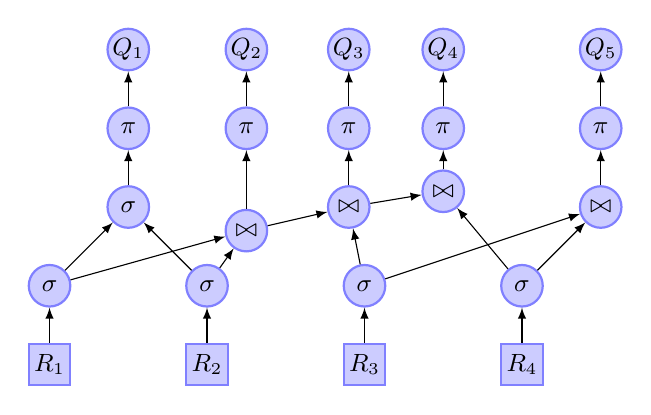
\begin{tikzpicture}[
every node/.style  = {fill=blue!20,draw=blue!50,thick,
	minimum size=1.5em,inner sep=0pt,font=\small},
circle_node/.style={circle},
rec_node/.style={rectangle},
edge from parent/.style={->,draw},
every label/.append style={font=\scriptsize},
>=latex]
  
    \node[rec_node] (r1) at (0, 0) {$R_1$};
    \node[rec_node] (r2) at (2, 0)  {$R_2$};
    \node[rec_node] (r3) at (4, 0) {$R_3$};
	\node[rec_node] (r4) at (6, 0) {$R_4$};
	
	\node[circle_node] (op1) at (0, 1) {$\sigma$};
	\node[circle_node] (op2) at (2, 1) {$\sigma$};
	\node[circle_node] (op3) at (4, 1) {$\sigma$};
	\node[circle_node] (op4) at (6, 1) {$\sigma$};
	
	\node[circle_node] (op5) at (1, 2) {$\sigma$};
	\node[circle_node] (op6) at (2.5, 1.7) {$\bowtie$};
	\node[circle_node] (op7) at (3.8, 2) {$\bowtie$};
	\node[circle_node] (op8) at (5, 2.2) {$\bowtie$};
	\node[circle_node] (op9) at (7, 2) {$\bowtie$};
	
	\node[circle_node] (op10) at (1, 3) {$\pi$};
	\node[circle_node] (op11) at (2.5, 3) {$\pi$};
	\node[circle_node] (op12) at (3.8, 3) {$\pi$};
	\node[circle_node] (op13) at (5, 3) {$\pi$};
	\node[circle_node] (op14) at (7, 3) {$\pi$};
	
	\node[circle_node] (q1) at (1, 4) {$Q_1$};
	\node[circle_node] (q2) at (2.5, 4) {$Q_2$};
	\node[circle_node] (q3) at (3.8, 4) {$Q_3$};
	\node[circle_node] (q4) at (5, 4) {$Q_4$};
	\node[circle_node] (q5) at (7, 4) {$Q_5$};

    \draw[->] (r1) -- (op1);
	\draw[->] (r2) -- (op2);
	\draw[->] (r3) -- (op3);
	\draw[->] (r4) -- (op4);
	
	\draw[->] (op1) -- (op5);
	\draw[->] (op1) -- (op6);
	\draw[->] (op2) -- (op5);
	\draw[->] (op2) -- (op6);
	\draw[->] (op3) -- (op7);
	\draw[->] (op3) -- (op9);
	\draw[->] (op4) -- (op8);
	\draw[->] (op4) -- (op9);
	
	\draw[->] (op5) -- (op10);
	\draw[->] (op6) -- (op11);
	\draw[->] (op6) -- (op7);
	\draw[->] (op7) -- (op12);
	\draw[->] (op7) -- (op8);
	\draw[->] (op8) -- (op13);
	\draw[->] (op9) -- (op14);
	
	\draw[->] (op10) -- (q1);
	\draw[->] (op11) -- (q2);
	\draw[->] (op12) -- (q3);
	\draw[->] (op13) -- (q4);
	\draw[->] (op14) -- (q5);
	
\end{tikzpicture}